\section{A New Design for Building Secure Virtualization Systems}
\label{sec.design}

This section discusses how to use the observation
 that ``commonly used kernel paths'' contain fewer bugs
(Section {\ref{sec.metric}) to build secure virtualization systems.
A key idea of our design is that all code \emph{including the complex part
of the operating system API} should have a very small TCB that accesses only
commonly used kernel paths.
Any complex or possibly risky system functions
are reimplemented by our own code within a sandbox. In this manner, any bugs
or failures within the implementation of these complex system functions
are contained by the sandbox. As a result, untrusted code would not be able to
and trigger sensitive and risky portions of the kernel.


\begin{figure}%[h]
\centering
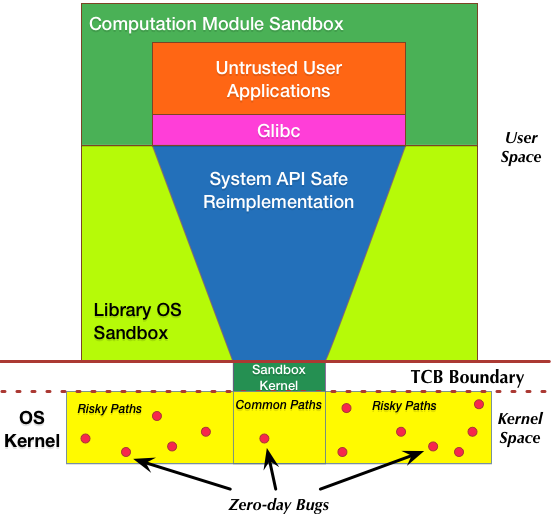
\includegraphics[width=1.0\columnwidth]{diagram/lind_secure_design_new.png}
\caption{``Safe-Reimplementation'' design to ensure predictable execution of untrusted user codes despite existing potential zero-day bugs within the OS kernel.}
\label{fig:design}
\end{figure}

\subsection{Architecture}

To execute untrusted applications in a manner that will not trigger bugs
in the underlying OS kernel, %and cause damage to other parts of the system,
we must build a virtualization system that can provide isolation and
containment for any improper operations.
One approach to building such a system is to place it entirely in the userspace,
and to restrict both the size of the sandbox kernel and its access to the
OS kernel (Figure \ref{fig:design}).
This approach has advantages over others that require modifications to
the OS kernel itself, as it avoids the risk of threat escalation. If modified modules
are inside the OS kernel, they have kernel privileges that could allow attacks
on the underlying system, as well as any applications run on top of it.

As shown in Figure \ref{fig:design}, our secure virtualization system
has two components.
The first is a computation module, which performs functions like type checking,
object creation, and garbage collection. The second is a library OS that
serves requests to access the OS kernel.
Together these components can complete the requirements of running user code.
First the system invokes the computation module to perform its operations,
and, if there are, the computation module directs those requests to our
library OS.The library OS then responds to the system call requests and
return results to the user code, if the requests are granted.

\subsubsection{The Computation Module}

Our secure system should be able to support and run legacy applications,
and execute binary code compiled from unmodified source code on popular hardware architecture,
like x86 architecture. Providing an execution environment that can run unmodified source code is
the main responsibility of the computation module. The key security issue of executing system calls
without triggering OS kernel bugs is left to the library OS module.

\subsubsection{The Library OS Module}

The Library OS module is the core of our virtualization system. It is comprised
of two parts: a sandbox kernel that provides access to basic but critical
system calls, and a system API safe reimplementation that implements more
complex calls. \lois{a short definition of what a "complex" call may be needed.}

The sandbox kernel forms the only addition to the TCB of our system.\lois{Is it the
only addition to the TCB or the only component of the TCB? If the "contents" of
the TCB were addressed up to this point, I don't remember seeing it.}  We
make this system extremely small and simple so that it is easy to verify its
security. \lois{How does it verify its secuirty? Does its small size alone do that?}
 The sandbox code provides an API that performs
a few critical system calls with the most basic parameters.  For example,
programs need some mechanism to write data to the file system
and communicate with the network.  The kernel's goal is to provide the ability
to do so, while utilizing the most simplistic calls possible with the most
basic arguments. For example, the file system API only need to provide a way
to write data to storage.  It need not provide a directory abstraction, the
concept of file permissions, links, or even the concept of multiple files.

%It should have a set of capabilities that enable the construction of essential and more complicated functions.
%For example, the sandbox kernel capabilities should include basic functions for network,
%file system I/O, lock, thread, and namespace. It also needs to have access to the OS kernel through system calls.
%In developing our design, we leveraged our verified hypothesis that commonly used kernel paths contain fewer bugs.
%Thus, the system calls we allow in our sandbox kernel are common calls, like file open, read, write, and close.
%Furthermore, the set of arguments used for each call is also highly restricted.

The system API safe reimplementation is a set of more complicated system calls
derived from functions within the sandbox kernel. \lois{Yiwen and I discussed this
somewhat awkward sentence. It is better now but could probably be tweaked more}
We reimplement those system calls because we do not want this potentially risky user code
to have direct access to the underlying OS kernel.
Instead, our reimplementation layer serves as a mediator between the user code
and the OS kernel. The reimplementation is safe
because the reconstructed call is isolated in a sandbox, and the code for the
reimplementation is written in a memory-safe programming language.
\lois{again, Yiwen and I discussed this idea of "memory-safe programming language"
I found it a bit awkward and so I re-wrote as it appears above. Not sure itv works}
With this design, even if there are bugs in the function reimplementation,
they cannot escape from the sandbox and will not reach the underlying OS kernel.

Here is an example of how this reimplementation would work with the symbolic link function.
If there is a bug in this function, rather than rely on the kernel code paths
for symbolic links, our sandbox system will implement the incorrect behavior.
The program will not be forced to quit, but by reimplementing it in the sandbox,
the code does not have privileged access to the system as the OS kernel does,
This will not result in a security issue, but instead, the application will just fail.

With the computation module and the library OS module, unmodified user code is able to run on top of our designed system.
It is important to note that our design does not rely on any specific technique or tool, and it is possible
to choose from several different techniques that fit well with the users' specific needs or requirements.

Based on this general system, we implemented a prototype security system based on a controlled kernel access that we called Lind.
Below we offer a short explanation of one design feature: the use of dual sandboxes. The following section offers a more detailed descripion of Lind's design and implementation.

\subsection{Discussion: Our Design Choice}

In reviewing our design, some fundamental questions could be raised about the dual sandbox design choice.
Why is one not enough? And, if two is good, why not use three or more?
The answer to the first question is that the kernel interface is extremely rich and hard to protect.
In order to have minimal impact on the kernel, as well as provide sufficient API for legacy applications,
we need to have one sandbox focuses on protecting the kernel and providing POSIX API,
while a second sandbox focuses on efficiently executing applications.
So our approach includes two sandboxes, one as the computation module,
and the other one as library OS module. As to the second question,
which could be rephrased as ``why not sandbox the sandbox kernel TCB and get more security?,''
the lowest level sandbox eventually must have some fundamental,
even if  limited access to system resources, such as memory, and storage, threads.
So even if we were to sandbox the sandbox kernel and have additional sandboxes,
the one at the bottom level will still access the OS kernel in a similar way.
Thus, having multiple sandboxes does not provide any extra security benefits.
